%-------------------------------------------------------------------------------
% cookbook_banks
%-------------------------------------------------------------------------------
%
% \file        cookbook_banks.tex
% \library     Documents
% \author      Chris Ahlstrom
% \date        2015-07-12
% \update      2016-02-22
% \version     $Revision$
% \license     $XPC_GPL_LICENSE$
%
%     Provides the cookbooks_banks section of yoshimi-cookbook.tex.
%
%-------------------------------------------------------------------------------

\section{Banks and General MIDI}
\label{sec:cookbook_banks}

   Banks are discussed quite heavily in the user manual \cite{yoshimidoc}.
   Banks have evolved quite a bit in \textsl{Yoshimi}, and are
   a powerful way to manage instruments, and more amenable to automation
   than ever.

   In this section, we will attempt to set up a basic bank that is
   compliant with the General MIDI specification.  In order to do so, we
   will cherry pick instruments from the package that is provided when
   \textsl{Yoshimi} is installed, renaming them as needed to fit into the
   appropriate General MIDI slot.

   One problem is the selection of the \textsl{best} instrument for a given
   General MIDI program number.  There are simply too many to be able to
   evaluate them all.

   For this recipe, the \texttt{banks} and \texttt{presets} will
   be stored in the following directories of this project:
   \index{directories!demo bank}
   \index{directories!GM basic bank}
   \index{directories!demo presets}

   \begin{verbatim}
      yoshimi/banks
      yoshimi/banks/demo
      yoshimi/banks/gm-basic
      yoshimi/presets
   \end{verbatim}

\subsection{Creating a Basic GM Bank}
\label{subsec:cookbook_banks_basic_gm}

   Creating even a basic General MIDI bank is beset with issues, even if one
   has at hand a large number of pre-built instruments.

   First, what is the purpose of the General MIDI specification?
   \index{GM}
   \index{General MIDI}
   To provide a
   dependable set of instruments so that tunes will sound basically similar
   on different GM-compliant synthesizers.  That's about it.  It doesn't
   guarantee that the sounds are consistent, nor does it guarantee that they
   are all of high quality.  The "FX", "Lead", and "Pad" instruments provide
   ambiguous descriptions that a wide range of sounds might fit.
   Getting a complete and high-quality set of sounds is extremely difficult.

   Second, evaluating a large number of pre-built \textsl{Yoshimi} and
   \textsl{ZynAddSubFX} instruments takes a lot of
   work.  We'd done some of this work for another project, and never
   finished.  Nor is the naming of such instruments all that helpful; many
   of the file-names are misleading.  Finding decent matches for a GM
   instrument takes time.

   Third, there are many GM instruments for which we've been able to find no
   good \textsl{ZynAddSubFX}/\textsl{Yoshimi} counterpart.  The only options
   are to pick a tolerable match, build a tolerable match oneself, or just
   plug in any old sound and wait for others to step up.

   Nonetheless, let's forge ahead.  The project file
   \texttt{contrib/instrument.ods}
   \index{GM!spreadsheet}
   is a \textsl{LibreOffice} spreadsheet
   that represents some research in finding GM-compatible instruments.
   It's pretty bad; maybe 50\% useful.

   We converted it to \texttt{contrib/gmcopy} to copy the files
   into the project directory \texttt{yoshimi/banks/gm/basic}.
   We show the banks in table~\ref{table:gm_basic_files}
   for convenience.

   \index{GM!table}

%-------------------------------------------------------------------------------
% gm_basic_table
%-------------------------------------------------------------------------------
%
% \file        gm_basic_table.tex
% \library     Documents
% \author      Chris Ahlstrom
% \date        2015-06-15
% \update      2015-07-18
% \version     $Revision$
% \license     $XPC\_GPL\_LICENSE$
%
%     Provides the concepts.
%
%-------------------------------------------------------------------------------

\label{table:gm_basic_files}
\begin{longtable}{|l l|}

\caption{GM Basic Files} \\

\hline
   \textbf{General MIDI Instrument} &
      \textbf{Yoshimi Instrument Used} \\
\hline
\endfirsthead

\hline
   \textbf{General MIDI Instrument} &
      \textbf{Yoshimi Instrument Used} \\
\hline
\endhead

\hline
   Continued next page & \\
\hline
\endfoot

\hline
   End of table & \\
\hline
\endlastfoot

   \textbf{0001-Acoustic Grand Piano} &
      SynthPiano/0033-Analog Piano 1 \\
   \textbf{0002-Bright Acoustic Piano} &
      SynthPiano/0034-Analog Piano 2 \\
   \textbf{0003-Electric Grand Piano} &
      SynthPiano/0143-Space Piano \\
   \textbf{0004-Honky-tonk Piano} &
      SynthPiano/0068-Synth Piano 3 fat \\
   \textbf{0005-Electric Piano 1} &
      Rhodes/0002-DX Rhodes 2 \\
   \textbf{0006-Electric Piano 2} &
      Rhodes/0007-Dig Rhodes \\
   \textbf{0007-Harpsichord} &
      olivers100/0026-Harpsichord \\
   \textbf{0008-Clavinet} &
      Misc Keys/0060-Clavinet 1 \\
   \textbf{0009-Celesta} &
      Bells/0002-Music\_Box \\
   \textbf{0010-Glockenspiel} &
      Bells/0011-Glass bells \\
   \textbf{0011-Music Box} &
      Bells/0013-Tiny bells \\
   \textbf{0012-Vibraphone} &
      Chromatic Percussion/0045-Vibes no\_trem \\
   \textbf{0013-Marimba} &
      Chromatic Percussion/0056-FM marimba \\
   \textbf{0014-Xylophone} &
      Will\_Godfrey\_Collection/0001-Xylophone \\
   \textbf{0015-Tubular Bells} &
      Chromatic Percussion/0097-Marimba 3 \\
   \textbf{0016-Dulcimer} &
      Plucked/0004-Plucked 4 \\
   \textbf{0017-Drawbar Organ} &
      Organ/0001-Organ 1 \\
   \textbf{0018-Percussive Organ} &
      Organ/0012-Organ 12 \\
   \textbf{0019-Rock Organ} &
      Organ/0068-Square Organ \\
   \textbf{0020-Church Organ} &
      Organ/0061-Great Organ \\
   \textbf{0021-Reed Organ} &
      Reed\_and\_Wind/0039-Reed 7 \\
   \textbf{0022-Accordion} &
      Organ/0097-Accordion Pad 1 \\
   \textbf{0023-Harmonica} &
      Reed\_and\_Wind/0099-Sharp Reed \\
   \textbf{0024-Tango Accordion} &
      Organ/0101-Accordion 1 \\
   \textbf{0025-Acoustic Guitar nylon} &
      Piano/0144-Soft Piano1 \\
   \textbf{0026-Acoustic Guitar steel} &
      Guitar/0065-Clean Guitar1 \\
   \textbf{0027-Electric Guitar jazz} &
      Guitar/0066-Electric Guitar \\
   \textbf{0028-Electric Guitar clean} &
      Guitar/0133-Smooth Guitar \\
   \textbf{0029-Electric Guitar muted} &
      Guitar/0035-Short \\
   \textbf{0030-Overdriven Guitar} &
      Guitar/0042-Trash Guitar 3 \\
   \textbf{0031-Distortion Guitar} &
      Guitar/0005-Dist Guitar 5 \\
   \textbf{0032-Guitar harmonics} &
      Laba170bank/0028-PianoBell \\
   \textbf{0033-Acoustic Bass} &
      Will\_Godfrey\_Collection/0045-Steel Bass \\
   \textbf{0034-Electric Bass finger} &
      Bass/0009-Electric bass 1 \\
   \textbf{0035-Electric Bass pick} &
      Bass/0041-Electric\_Bass \\
   \textbf{0036-Fretless Bass} &
      Bass/0050-Fretless Bass \\
   \textbf{0037-Slap Bass 1} &
      Rhodes/0042-Hard Rhodes1 \\
   \textbf{0038-Slap Bass 2} &
      olivers-100/0018-Bass Guitar - Slap \\
   \textbf{0039-Synth Bass 1} &
      Bass/0013-FM rubber bass \\
   \textbf{0040-Synth Bass 2} &
      Bass/0024-Moog bass \\
   \textbf{0041-Violin} &
      Strings/0051-Synth Violin 2 Fat \\
   \textbf{0042-Viola} &
      Strings/0051-Synth Violin 2 Fat \\
   \textbf{0043-Cello} &
      Strings/0051-Synth Violin 2 Fat \\
   \textbf{0044-Contrabass} &
      Bass/0005-Bass 5 \\
   \textbf{0045-Tremolo Strings} &
      Strings/0001-Saw Strings 1 \\
   \textbf{0046-Pizzicato Strings} &
      Strings/0003-Saw Strings 3 \\
   \textbf{0047-Orchestral Harp} &
      Pads/0065-Soft Pad \\
   \textbf{0048-Timpani} &
      Noises/0018-Gun \\
   \textbf{0049-String Ensemble 1} &
      VDX/0065-Strings \\
   \textbf{0050-String Ensemble 2} &
      folderol collection/0029-Full Strings \\
   \textbf{0051-Synth Strings 1} &
      Strings/0010-Strings Pad1 \\
   \textbf{0052-Synth Strings 2} &
      Strings/0014-Strings Pad5 \\
   \textbf{0053-Choir Aahs} &
      Choir\_and\_Voice/0001-AHH Choir 1 \\
   \textbf{0054-Voice Oohs} &
      Choir\_and\_Voice/0004-Voice OOH \\
   \textbf{0055-Synth Voice} &
      Choir\_and\_Voice/0005-Choir Pad1 \\
   \textbf{0056-Orchestra Hit} &
      Misc/0010-Industrial orchestra \\
   \textbf{0057-Trumpet} &
      Leads/0027-Prophet horn 2 \\
   \textbf{0058-Trombone} &
      Brass/0033-Analog Brass 1 \\
   \textbf{0059-Tuba} &
      Brass/0001-FM Thrumpet \\
   \textbf{0060-Muted Trumpet} &
      Synth/0001-Soft Synth 1 \\
   \textbf{0061-French Horn} &
      Brass/0034-Analog Brass 2 \\
   \textbf{0062-Brass Section} &
      Brass/0007-Synth Brass 5 \\
   \textbf{0063-Synth Brass 1} &
      Brass/0003-Synth Brazz 1 \\
   \textbf{0064-Synth Brass 2} &
      Brass/0004-Synth Brazz 2 \\
   \textbf{0065-Soprano Sax} &
      Reed\_and\_Wind/0066-Fat Reed2 \\
   \textbf{0066-Alto Sax} &
      Reed\_and\_Wind/0065-Fat Reed1 \\
   \textbf{0067-Tenor Sax} &
      Reed\_and\_Wind/0037-Reed 5 \\
   \textbf{0068-Baritone Sax} &
      Reed\_and\_Wind/0099-Sharp Reed \\
   \textbf{0069-Oboe} &
      Reed\_and\_Wind/0040-Reed 8 \\
   \textbf{0070-English Horn} &
      Brass/0034-Analog Brass 2 \\
   \textbf{0071-Bassoon} &
      Will\_Godfrey\_Collection/0102-Bassoon \\
   \textbf{0072-Clarinet} &
      Reed\_and\_Wind/0006-Clarinet \\
   \textbf{0073-Piccolo} &
      Will\_Godfrey\_Collection/0071-Ocarina \\
   \textbf{0074-Flute} &
      Will\_Godfrey\_Collection/0057-Soft Flute \\
   \textbf{0075-Recorder} &
      Will\_Godfrey\_Collection/0059-Ocarina \\
   \textbf{0076-Pan Flute} &
      Will\_Godfrey\_Collection/0127-Pan Pipe \\
   \textbf{0077-Blown Bottle} &
      Will\_Godfrey\_Collection/0125-Bottle \\
   \textbf{0078-Shakuhachi} &
      Will\_Godfrey\_Collection/0125-Pan Pipe 32 \\
   \textbf{0079-Whistle} &
      Will\_Godfrey\_Collection/0027-Ghost Whistle \\
   \textbf{0080-Ocarina} &
      Flute/0071-Ocarina \\
   \textbf{0081-Lead 1 square} &
      Leads/0022-Square lead \\
   \textbf{0082-Lead 2 sawtooth} &
      Louigi\_Verona\_Workshop/0008-saw-lead \\
   \textbf{0083-Lead 3 calliope} &
      Leads/0018-Sine lead \\
   \textbf{0084-Lead 4 chiff} &
      chip/0018-Chiffer\_Chip \\
   \textbf{0085-Lead 5 charang} &
      Louigi\_Verona\_Workshop/0001-progressive-lead-1 \\
   \textbf{0086-Lead 6 voice} &
      Choir\_and\_Voice/0067-Vocal Morph 3 \\
   \textbf{0087-Lead 7 fifths} &
      chip/0017-SuperSquare1 \\
   \textbf{0088-Lead 8 bass lead} &
      Strings/0157-Dual Strings Oct2 \\
   \textbf{0089-Pad 1 new age} &
      Pads/0028-Ethereal \\
   \textbf{0090-Pad 2 warm} &
      Will\_Godfrey\_Companion/0019-Warm Square Swell \\
   \textbf{0091-Pad 3 polysynth} &
      Dual/0065-Dream of the Saw \\
   \textbf{0092-Pad 4 choir} &
      Alex\_J/0100-Choir Pad \\
   \textbf{0093-Pad 5 bowed} &
      The\_Mysterious\_Bank/0004-trance\_strings\_pad \\
   \textbf{0094-Pad 6 metallic} &
      The\_Mysterious\_Bank/0011-dreaming\_bells \\
   \textbf{0095-Pad 7 halo} &
      Alex\_J/RadioPulsePad \\
   \textbf{0096-Pad 8 sweep} &
      Pads/0011-lightbeam \\
   \textbf{0097-FX 1 rain} &
      The\_Mysterious\_Bank/0037-the\_rain \\
   \textbf{0098-FX 2 soundtrack} &
      The\_Mysterious\_Bank/0038-falling\_stars \\
   \textbf{0099-FX 3 crystal} &
      Will\_Godfrey\_Companion/0006-Tinkle Bell \\
   \textbf{0100-FX 4 atmosphere} &
      The\_Mysterious\_Bank/0038-the\_starting\_machine \\
   \textbf{0101-FX 5 brightness} &
      Noises/0014-droplets for chords \\
   \textbf{0102-FX 6 goblins} &
      Noises/0002-Ioioioioioi \\
   \textbf{0103-FX 7 echoes} &
      Noises/0072-Cave Gates \\
   \textbf{0104-FX 8 sci-fi} &
      The\_Mysterious\_Bank/0031-etrange\_sound \\
   \textbf{0105-Sitar} &
      olivers-100/0019-FM Sitar \\
   \textbf{0106-Banjo} &
      olivers-100/0016-Banjoey \\
   \textbf{0107-Shamisen} &
      Plucked/0034-Plucked String2 \\
   \textbf{0108-Koto} &
      Plucked/0003-Plucked 3 \\
   \textbf{0109-Kalimba} &
      Plucked/0001-Plucked 1 \\
   \textbf{0110-Bagpipe} &
      Reed\_and\_Wind/0033-Reed 1 \\
   \textbf{0111-Fiddle} &
      Laba170bank/0055-DevilsFiddle2 \\
   \textbf{0112-Shanai} &
      Reed\_and\_Wind/0035-Reed 3 \\
   \textbf{0113-Tinkle Bell} &
      Bells/0011-Glass bells \\
   \textbf{0114-Agogo} &
      The\_Mysterious\_Bank/0028-snare \\
   \textbf{0115-Steel Drums} &
%     C\_Ahlstrom/Add\_Pseudo\_Steel\_Drums\_2 \\   Found one even better!
      olivers-100/0029-Steel Drums \\
   \textbf{0116-Woodblock} &
      The\_Mysterious\_Bank/0028-snare \\
   \textbf{0117-Taiko Drum} &
      The\_Mysterious\_Bank/0028-snare \\
   \textbf{0118-Melodic Tom} &
      demo/Melodic\_Tom\_from\_Nat\_drum\_kit \\
   \textbf{0119-Synth Drum} &
      The\_Mysterious\_Bank/0028-snare \\
   \textbf{0120-Reverse Cymbal} &
      The\_Mysterious\_Bank/0028-snare \\
   \textbf{0121-Guitar Fret Noise} &
      The\_Mysterious\_Bank/0028-snare \\
   \textbf{0122-Breath Noise} &
      The\_Mysterious\_Bank/0028-snare \\
   \textbf{0123-Seashore} &
      Noises/0008-Wind and Surf \\
   \textbf{0124-Bird Tweet} &
      The\_Mysterious\_Bank/0028-snare \\
   \textbf{0125-Telephone Ring} &
      The\_Mysterious\_Bank/0028-snare \\
   \textbf{0126-Helicopter} &
      The\_Mysterious\_Bank/0028-snare \\
   \textbf{0127-Applause} &
      The\_Mysterious\_Bank/0028-snare \\
   \textbf{0128-Gunshot} &
      Noises/0018-Gun \\
   \textbf{0129-Drum Kit} &
      C\_Ahlstrom/Natural\_Drum\_Kit\_Basic \\
\end{longtable}

%-------------------------------------------------------------------------------
% vim: ts=3 sw=3 et ft=tex
%-------------------------------------------------------------------------------


   Presumably, this basic bank could be improved enough to be useful
   for most music.  Alternative (and better) banks could be created, as
   well.

   One thing to note about the instruments.  When copied from the original
   directory to the \texttt{gm-basic} directory, each instrument copied
   retains its name, of course.  To make it less confusing to use in
   \textsl{Yoshimi}, then, one should rename each instrument to its GM name.
   To do that, right click on the name, change it, and then save the
   instrument to the same file from which it was loaded.  Be careful!
   It is easy to make a mistake!  

   And we have not yet renamed any of them!

\subsection{Root Paths}
\label{subsec:cookbook_banks_root_paths}

   The first thing to do is to add the yoshimi-cookbook \texttt{banks}
   directory to your setup.

   Run \textsl{Yoshimi}, and navigate the following user-interface path:
   \textsl{Menu / Instrument / Show Root Paths ...}

   Then click \textbf{Add root directory...}.  Navigate to where the
   yoshimi-cookbook project is stored and add the \texttt{yoshimi/banks}
   directory.  The result should be something like the following:

\begin{figure}[H]
   \centering 
   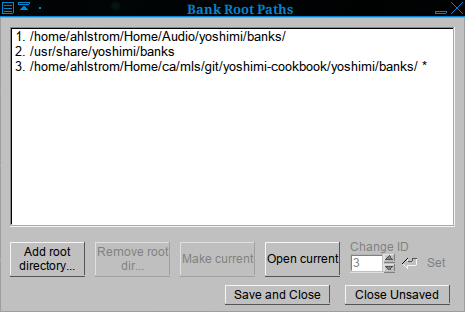
\includegraphics[scale=1.0]{menu/Instrument/bank_root_paths.png}
   \caption{Bank Root Paths}
   \label{fig:cookbook_bank_root_paths}
\end{figure}

   Click on the new directory.
   \index{GM!bank}
   It has ID = 3 in that diagram.  We will refer to this value as
   the "banks path".
   Now click the \textbf{Make current} button.
   Verify that it now has the asterisk. 
   Click the \textbf{Save and Close} button.

   Now let's open the "gm-basic" bank.
   Run \textsl{Yoshimi}, and navigate the following user-interface path:
   \textsl{Menu / Instrument / Show Banks ...}

   In the matrix of banks, you should see "gm-basic" somewhere.
   (We also have a "demo" bank in place.)

\begin{figure}[H]
   \centering 
   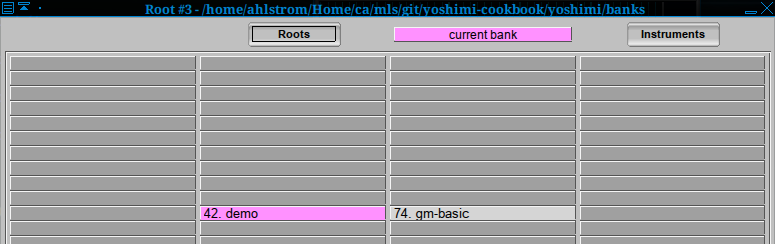
\includegraphics[scale=0.75]{menu/Instrument/demo_gm-basic_banks.png}
   \caption{Two Banks, Demo and Basic GM}
   \label{fig:cookbook_bank_demo_gm_basic}
\end{figure}
   
   \index{directories!GM basic bank}
   Click on the "gm-basic" bank.  The larger dialog below will be shown.
   \index{current bank}
   Note that this action also makes "gm-basic" the current bank.
   This setting will be preserved across a restart of \textsl{Yoshimi}.

\begin{figure}[H]
   \centering 
   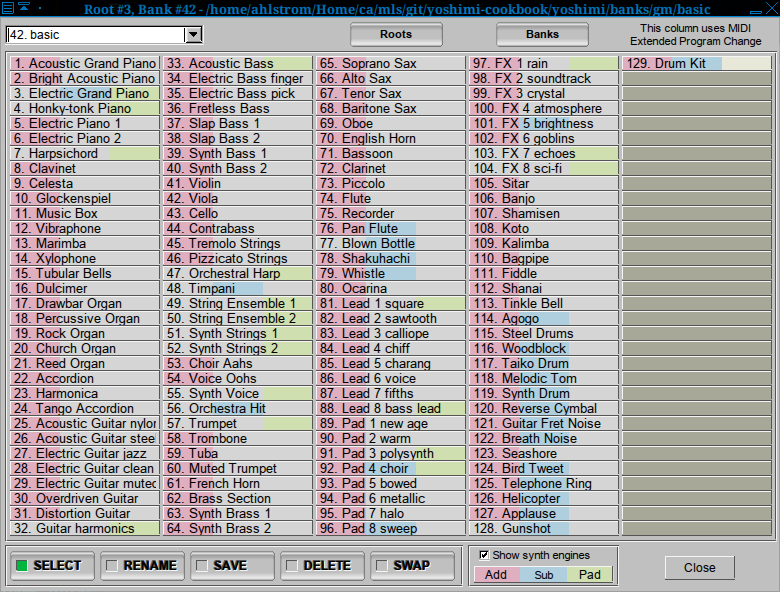
\includegraphics[scale=0.85]{menu/Instrument/banks_gm_basic.png}
   \caption{A General MIDI Basic Bank}
   \label{fig:cookbook_bank_basic_bank}
\end{figure}

   Remember that these banks have GM names; the original files used to
   create each one are listed in the spreadsheet mentioned in the previous
   section.

   \index{drum kit}
   \index{GM!drum kit}
   Also note the drum kit, with an ID of 129.  Normally, drum kits might be
   stored in a bank of drum kits, but here we have a GM-compliant drum kit,
   compliant in the sense that most of the keys are mapped correctly, and
   all keys will play \textsl{something}.

\subsection{Using a Basic GM Bank}
\label{subsec:cookbook_banks_using_basic_bank}

   \index{current root}
   Once the current root path has been set (e.g. to
   \texttt{~/yoshimi-cookbook/yoshimi/banks}) and
   \index{current bank}
   the current bank has been set (e.g. to \texttt{gm-basic}),
   then a MIDI file can select instruments 1 to 128 from the
   current bank using a Program Change event followed by the desired
   instrument's number re 0.

   The bank and root paths can be saved in the \textsl{Yoshimi} state.
   But the MIDI file can also start with bank-selection events, and change
   the current bank using Bank Select LSB (CC32) and Bank Select MSB (CC0)
   events.

%-------------------------------------------------------------------------------
% vim: ts=3 sw=3 et ft=tex
%-------------------------------------------------------------------------------
